\subsection{Funktionsorientierter Test (Black-Box-Test)}
\label{sec:Kap-11-1-4}

Die Testfälle beim funktionsorientiertem Test werden ausschließlich aufgrund der Spezifikation erstellt. 
Black-Box heißt, dass der Programmcode selbst dem Tester nicht bekannt ist bzw. bekannt sein muss. Er spielt bei der Bestimmung der Testfälle jedenfalls keine Rolle.

Mögliche Ziele beim funktionsorientiertem Test sind:
\begin{itemize}
	\item Funktionsüberdeckung: jede spezifizierte Funktion wird einmal aktiviert,
	\item Ausgabeüberdeckung: jede Ausgabe wird wenigstens einmal erzeugt, 
	\item Ausnahmeüberdeckung: jede Ausnahme wird wenigstens einmal erzeugt.
\end{itemize}

Neben Einhaltung der funktionalen Anforderungen kann es auch um spezifizierte Leistungsanforderungen gehen, gerade auch unter ungünstigen Bedingungen
\linebreak %%% für Druck
(Belastungs\-tests).

Wie sollen die Testfälle ausgewählt werden? Natürlich könnte man zunächst vermuten: je mehr desto besser. Dies ist aber nicht die ganze Wahrheit, denn sehr viele Testfälle bedeuten auch sehr viel Testaufwand, der im Zweifel zu kostenaufwändig und insbesondere zu zeitaufwändig ist. Vielmehr ist es wichtig, dass die Testfälle ausgewählt werden, die mit einer gewissen Wahrscheinlichkeit Fehler aufdecken. Wenn Testfälle sich wahrscheinlich gleichen (deckt einer einen Fehler auf, dann der andere auch, und umgekehrt), so reicht die Betrachtung einer dieser Testfälle. Grob gesagt gilt für die Auswahl: Soviel wie nötig (existierende Fehler sollen gefunden werden) und dabei so wenig wie möglich (Effizienz).

Wir wollen als Beispiel den Algorithmus zur Berechnung des größten gemeinsamen Teilers (ggT) zweier natürlicher Zahlen aus Lektion~1 % TODO Lektion~\ref{sec:Lektion-1}
wieder aufgreifen. Abbildung~\ref{fig:flussdiagramm_in_Kap-11} zeigt das Flussdiagramm nochmal.

\begin{figure}[h!]
	\centering
	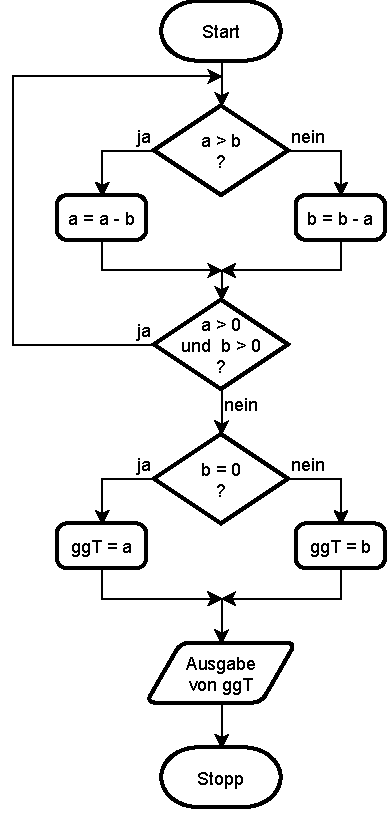
\includegraphics[scale=0.75]{Bilder/Kapitel-1/Abb-1-4.pdf}
	\caption[Der Euklidische Algorithmus als Flussdiagramm]{Ein Flussdiagramm, das den Euklidischen Algorithmus zur Be\-rechnung des größten gemeinsamen Teilers (ggT) zweier positiver Ganzzahlen grafisch darstellt}
	\label{fig:flussdiagramm_in_Kap-11}
\end{figure}


\minisec{Äquivalenzklassen}

Wenn man vermuten kann, dass ein Programm für zwei unterschiedliche Eingaben entweder in beiden Fällen korrekt läuft oder in beiden Fällen einen Fehler aufweist, so reicht es, eine der beiden Eingaben zu testen.

\vspace{1mm} %%% für Druck

Beispiel ggT-Algorithmus aus Abbildung~\ref{fig:flussdiagramm_in_Kap-11}: % TODO Kapitel~\ref{sec:Kap-2.1}:

\vspace{1mm} %%% für Druck

mögliche Äquivalenzklassen:

\begin{addmargin}[25pt]{25pt}
	$a>b>1$, \dasHeisst alle Werte von $a$ und $b$, für die $a>b>1$ gilt.
	
	$b>a>1$
	
	$a=b>1$
	
	$a=1$
	
	$b=1$
	
	$a=b=1$
\end{addmargin}

Man nennt diese Eingaben dann äquivalent und betrachtet entsprechende Äqui\-valenz\-klassen von Testfällen (streng genommen sind es keine Äquivalenzklassen, denn sie sind nicht notwendigerweise disjunkt).

\vspace{2mm} %%% für Druck

\minisec{Grenzwertanalyse}

An den Grenzwerten treten häufig Fehler auf. Die Grenzwerte können sowohl technischer Natur sein, also zum Beispiel die Darstellbarkeit der betroffenen Zahlen berühren. Oder aber sie sind durch den implementierten Algorithmus begründet.

\vspace{1mm} %%% für Druck

Beispiel ggT-Algorithmus:

\begin{addmargin}[25pt]{25pt}
	$a, b$ sehr groß
	
	$a,b$ sehr klein
\end{addmargin}

Die Grenzwertanalyse ist insbesondere relevant bei reellwertigen Eingaben.

\vspace{2mm} %%% für Druck

\minisec{Ursache-Wirkungsgraph}

Das ist bei Black-Box-Verfahren weniger einfach, weil die Programmstruktur nicht mit einbezogen werden darf. Es geht darum Eingaben zu finden, die bestimmte Ausgaben und insbesondere besondere Reaktionen wie Ausnahmen erzeugen.

\vspace{1mm} %%% für Druck

Beispiel ggT-Algorithmus:

\begin{addmargin}[25pt]{25pt}
	$a,b$ teilerfrei
	
	$a$ Vielfaches von $b$
	
	$b$ Vielfaches von $a$
\end{addmargin}

\vspace{2mm} %%% für Druck

\minisec{Ungültige Eingaben}

Beispiel ggT-Algorithmus:

\begin{addmargin}[25pt]{25pt}
	$a= 0$
	
	$b<0$
\end{addmargin}
